\pdfminorversion=7
\documentclass[12pt,letterpaper]{article}

\usepackage[T1]{fontenc}
\usepackage[utf8]{inputenc}
\usepackage[american]{babel}
\usepackage{csquotes}

\usepackage[
    style=science,
    backend=biber,
    sorting=none,
    articletitle=true,
    url=false,
    doi=false,
    eprint=false,
    isbn=false
]{biblatex}
\addbibresource{references.bib}
\AtEveryBibitem{\clearlist{language}}

\usepackage{newtxtext,newtxmath}
\usepackage{microtype}
\usepackage{amsmath}
\usepackage{graphicx}
\usepackage{booktabs}
\usepackage[margin=0.92in,top=0.82in,bottom=0.95in,headsep=18pt,footskip=24pt]{geometry}
\usepackage[font=small,labelfont=bf,labelsep=period]{caption}
\usepackage{subcaption}
\usepackage{float}
\usepackage{afterpage}
\usepackage{array}
\usepackage{multirow}
\usepackage{setspace}
\usepackage{titlesec}
\usepackage{enumitem}
\usepackage{fancyhdr}
\usepackage{needspace}
\usepackage{etoolbox}
\usepackage[section]{placeins}
\usepackage{flafter}
\usepackage[table]{xcolor}

\definecolor{ClayLine}{HTML}{EEDBDD}
\definecolor{SumiInk}{HTML}{2D2426}
\definecolor{DustyTaupe}{HTML}{866A6D}

\usepackage[hidelinks]{hyperref}
\usepackage[switch]{lineno}

\color{SumiInk}
\setstretch{1.45}
\setlength{\parindent}{0pt}
\setlength{\parskip}{0.42em}
\setlength{\textfloatsep}{8pt plus 1pt minus 1pt}
\setlength{\floatsep}{7pt plus 1pt minus 1pt}
\setlength{\intextsep}{7pt plus 1pt minus 1pt}
\setlength{\abovecaptionskip}{5pt}
\setlength{\belowcaptionskip}{2pt}
\setlength{\tabcolsep}{9pt}
\renewcommand{\arraystretch}{1.14}
\captionsetup{justification=raggedright,singlelinecheck=false}
\setlist[itemize]{leftmargin=1.3em,itemsep=0.18em,topsep=0.25em}
\setcounter{topnumber}{3}
\setcounter{bottomnumber}{2}
\setcounter{totalnumber}{4}
\renewcommand{\topfraction}{0.92}
\renewcommand{\bottomfraction}{0.85}
\renewcommand{\textfraction}{0.08}
\renewcommand{\floatpagefraction}{0.8}
\setlength{\headheight}{24pt}
\emergencystretch=2em
\raggedbottom

\titleformat{\section}
  {\Large\sffamily\bfseries\color{SumiInk}}
  {\thesection}
  {0.6em}
  {}
  [\vspace{0.25em}\color{ClayLine}\titlerule]
\titleformat{\subsection}
  {\large\sffamily\bfseries\color{SumiInk}}
  {\thesubsection}
  {0.55em}
  {}
\titleformat{\subsubsection}
  {\normalsize\sffamily\bfseries\color{SumiInk}}
  {}
  {0em}
  {}
\titlespacing*{\section}{0pt}{1.3ex plus 0.4ex minus 0.2ex}{0.7ex}
\titlespacing*{\subsection}{0pt}{1.15ex plus 0.2ex minus 0.2ex}{0.45ex}
\titlespacing*{\subsubsection}{0pt}{0.9ex plus 0.15ex minus 0.1ex}{0.25ex}

\pretocmd{\subsubsection}{\needspace{4\baselineskip}}{}{}
\pretocmd{\subsection}{\needspace{5\baselineskip}}{}{}

\pagestyle{fancy}
\fancyhf{}
\fancyhead[L]{\footnotesize\sffamily\color{SumiInk} Violin Back Media Wall}
\fancyhead[R]{\footnotesize\sffamily\color{DustyTaupe}\nouppercase{\leftmark}}
\fancyfoot[C]{\footnotesize\sffamily\thepage}
\renewcommand{\headrulewidth}{0.35pt}
\renewcommand{\headrule}{\hbox to\headwidth{\color{ClayLine}\leaders\hrule height \headrulewidth\hfill}}
\renewcommand{\sectionmark}[1]{\markboth{#1}{}}

\makeatletter
\def\fps@figure{tbp}
\def\fps@table{tbp}
\makeatother

\begin{document}
\linenumbers
\thispagestyle{empty}

\begin{center}
    \vspace*{-0.6em}

    {\fontsize{20}{22}\selectfont\bfseries\color{SumiInk}
    Violin backs as restorative visual media for craft attention and practice motivation\par}

    \vspace{0.95em}

    {\normalsize\color{SumiInk}
    Alan N. Pham$^{1}$\par}

    \vspace{0.38em}

    {\small\color{DustyTaupe}
    $^{1}$AO Labs, Worcester, MA, USA\par}
\end{center}

\vspace{0.35em}
\noindent\textbf{Violin practice often begins before sound: with the player's willingness to approach the instrument again. Here we present \texttt{violin.aolabs.io}, a source-gated media wall restricted to five named instruments: the 1740 ``Ysaye'' Guarneri del Gesu, the 1742 ``Lord Wilton'' Guarneri del Gesu, the 1734 ``Spagnoletti'' Guarneri del Gesu, the 1710 ex-Vieuxtemps Stradivari, and a 1940 Carl G. Becker Sr. violin. The deliberately closed instrument set makes membership explicit, so the viewer no longer has to infer which objects belong. We argue that the violin back is not a secondary surface but a compact record of craft history, material selection, varnish, wear, ownership, and desire. Drawing on arts-and-health research, self-determination theory, neuroaesthetics, aesthetic-appreciation models, and music-practice research, we frame the wall as an environmental intervention for attention and practice re-entry. No clinical or user-outcome claim is made; the contribution is a source-backed design framework for treating selected violin backs as serious cultural, motivational, and attentional media.}

\newpage
\pagestyle{fancy}

\section{Introduction}

Violin practice is an unusually demanding form of self-regulation. The player must return repeatedly to slow correction, audible failure, body calibration, and delayed reward. This is why the environment around practice matters. A room, screen, notebook, stand, or digital surface can either add friction or reduce it. A visual media wall of violin backs addresses this problem from a simple premise: before a player practises sound, they may need to want to approach the instrument again.

The violin back is a powerful but underused object for this purpose. It is not the face that carries the f-holes and bridge, nor the scroll that signals decorative identity, nor the label that can invite authentication anxiety. It is a large, continuous maple field, shaped by arching, centre joint, flame, varnish, edgework, corner wear, and centuries of handling. The back is where the instrument becomes visibly bodily. It is a surface of curvature, density, shine, abrasion, repair, and memory.

The design question behind \texttt{violin.aolabs.io} is therefore narrow by intention: what happens when the site shows only the short, named set of violins specified for this revision? The restriction removes generic violin content and keeps attention on five instruments rather than a fluctuating catalogue. The result is not a shop, a maker index, or an educational explainer. It is a visual environment: a source-linked wall of the ``Ysaye'', ``Lord Wilton'', ``Spagnoletti'', ex-Vieuxtemps, and Becker instruments.

This paper develops the intellectual basis for that surface. We combine four bodies of evidence. First, arts-and-health research supports the broad relevance of arts engagement to well-being, while also requiring caution about causal and clinical claims~\cite{fancourt_arts_2019}. Second, self-determination theory suggests that sustained motivation depends on experiences of autonomy, competence, and relatedness rather than only external pressure~\cite{ryan_self_2000}. Third, models of aesthetic appreciation and neuroaesthetics show that visual experience integrates sensory features, emotion, valuation, knowledge, and meaning~\cite{leder_model_2004,chatterjee_neuroaesthetics_2014}. Fourth, music-practice research shows that expertise depends on repeated, effortful practice and on self-regulatory behaviour over time~\cite{ericsson_deliberate_1993,mcpherson_self_2001}. Together, these literatures suggest that a beautiful, source-backed visual environment may make practice more approachable without pretending to replace instruction, discipline, or clinical care.

\section{Results}

\subsection{A back-only wall changes the unit of attention}

The present implementation of \texttt{violin.aolabs.io} uses one closed gate. A record is admitted only if it belongs to one of the five named instruments specified for the public wall and the served media can be traced to the matching source page. The inspected source file contains five records in a closed \texttt{selectedViolins} array. The ex-Vieuxtemps and Becker records render direct public back images; the ``Ysaye'', ``Lord Wilton'', and ``Spagnoletti'' records render the public instrument images exposed by the supplied source pages because the corresponding isolated Tarisio photo routes are not stable hotlink targets.

\begin{figure}[H]
    \centering
    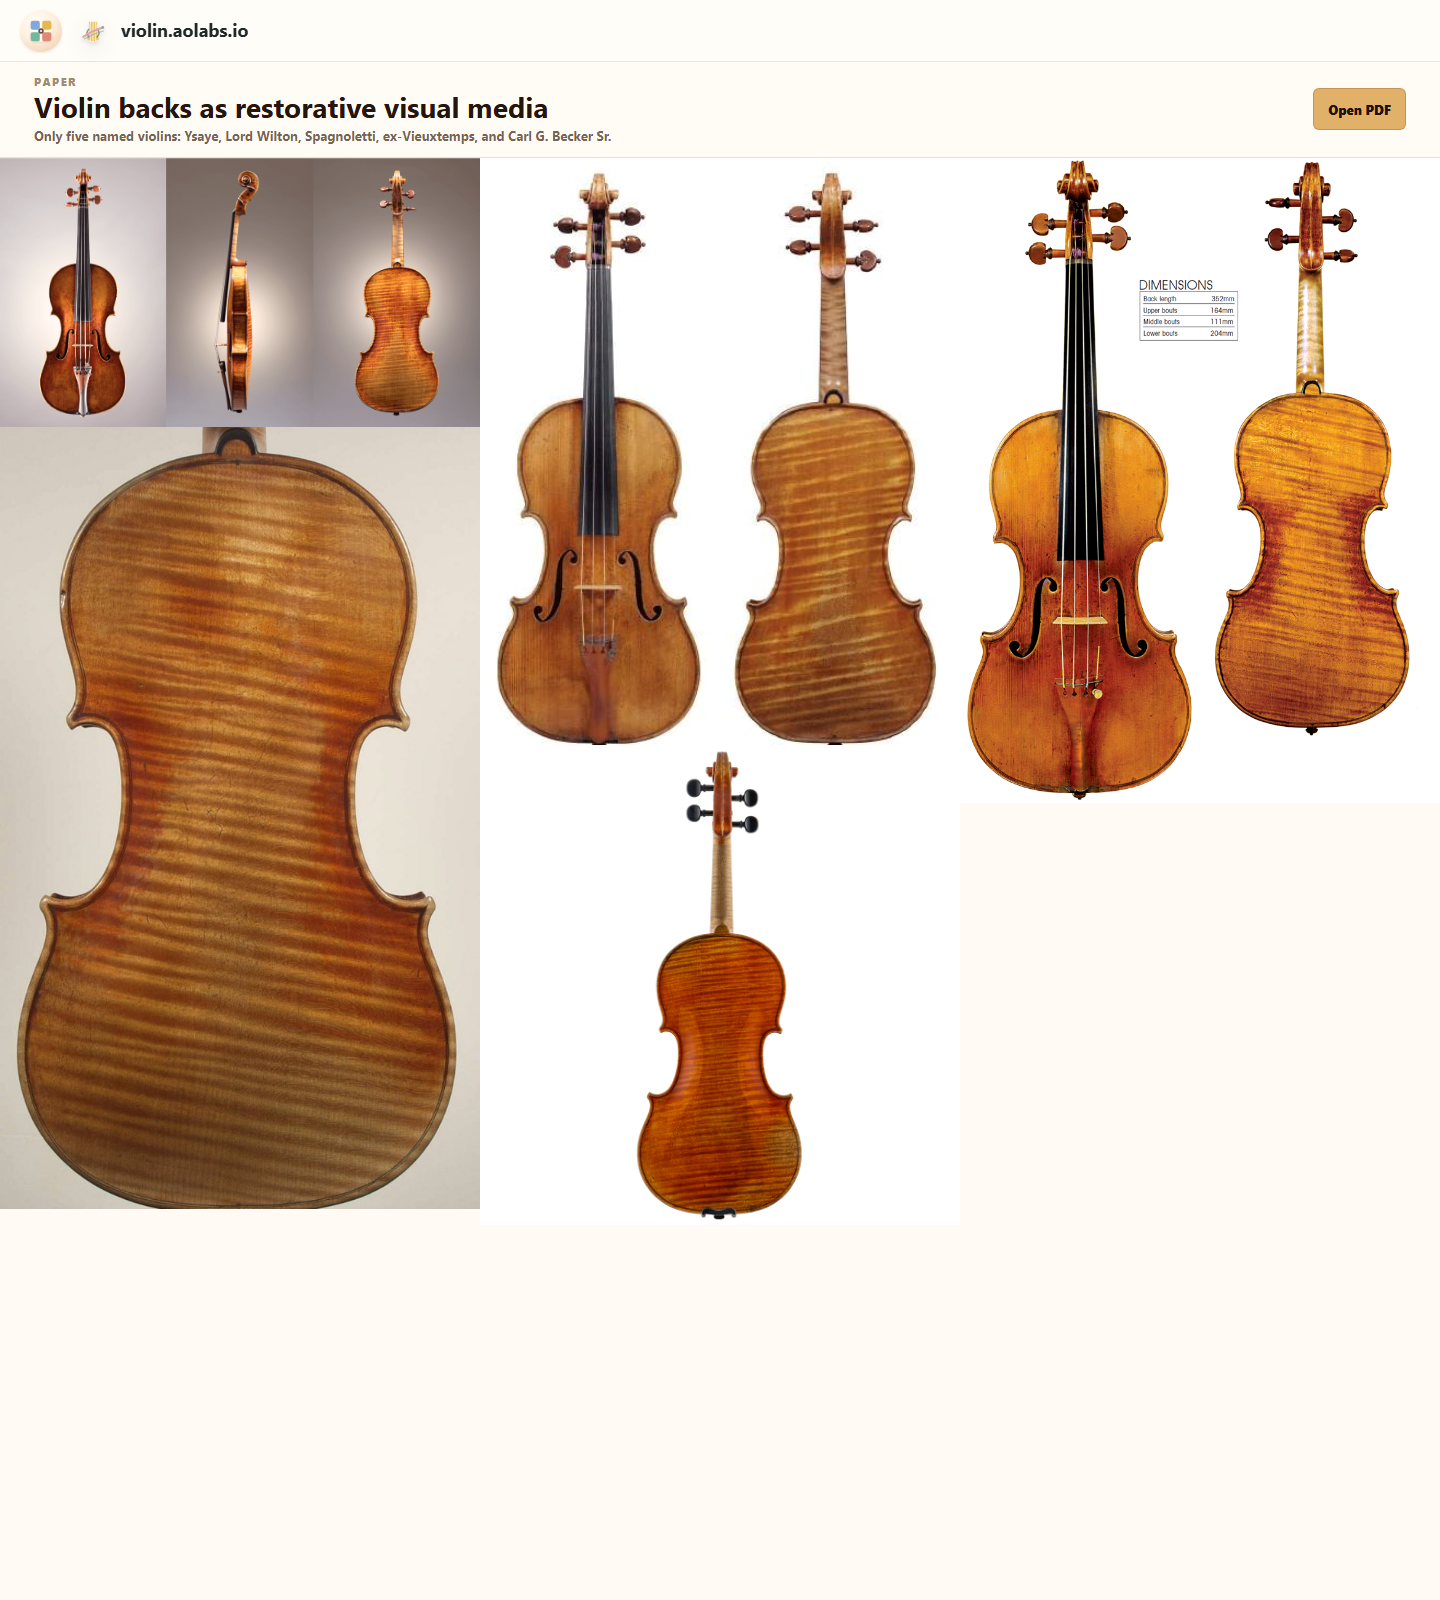
\includegraphics[width=\textwidth]{figures/fig01_violin_back_wall.png}
    \caption{Five-instrument source-gated wall. The deployed page is restricted to the ``Ysaye'', ``Lord Wilton'', ``Spagnoletti'', ex-Vieuxtemps, and Becker records, with source links preserved for provenance inspection.}
    \label{fig:wall}
\end{figure}

This restriction matters because it changes the visual object. A general violin gallery asks the viewer to recognise the violin as an instrument. A back-only wall asks the viewer to compare wood, curve, varnish, age, and makerly judgment. The violin is no longer a symbol of music in general; it becomes an array of specific material decisions.

\begin{table}[H]
    \centering
    \caption{Current source gate for \texttt{violin.aolabs.io}. The table reports the five records inspected in the application code on 24 May 2026.}
    \label{tab:source_gate}
    \begin{tabular}{p{0.30\textwidth}p{0.16\textwidth}p{0.42\textwidth}}
        \toprule
        Instrument & Accepted sources & Gate enforced \\
        \midrule
        1740 ``Ysaye'' Guarneri del Gesu & 1 tile & The Sasakawa Music Foundation page provides public instrument imagery, history, and descriptive context; Tarisio Cozio Archive record 40064 was checked for measurements and provenance~\cite{smf_ysaye_1740,tarisio_ysaye_1740}. \\
        1742 ``Lord Wilton'' Guarneri del Gesu & 1 tile & The Strad calendar page provides the public instrument image; Tarisio Cozio Archive record 40256 was checked for measurements and provenance~\cite{strad_lord_wilton_2024,tarisio_lord_wilton_1742}. \\
        1734 ``Spagnoletti'' Guarneri del Gesu & 1 tile & The Strad archive article is the supplied public source for the instrument and image record~\cite{strad_spagnoletti_1734}. \\
        1710 ex-Vieuxtemps Stradivari & 1 tile & Darnton \& Hersh provides the article record and public back image~\cite{darnton_vieuxtemps_1710}. \\
        Carl G. Becker Sr., Chicago, 1940 & 1 tile & SHAR Music provides the product record and public back image~\cite{shar_becker_1940}. \\
        \bottomrule
    \end{tabular}
\end{table}

The design therefore converts curation into an interface rule. An image is not accepted because it is violin-related; it is accepted because it belongs to the explicit five-instrument set. This is important for mental load. The viewer does not have to filter a large wall or decide whether a picture belongs. The page does that work before display.

\subsection{The violin back is a record of material choice}

The classical violin is a joined system of materials and geometries. The top is usually spruce; the back, ribs, and neck are usually maple. The selected source records keep that material fact attached to named objects rather than to generic violin imagery: the ``Ysaye'', ``Lord Wilton'', ``Spagnoletti'', ex-Vieuxtemps, and Becker pages each locate visual attention inside a specific instrument history~\cite{smf_ysaye_1740,tarisio_ysaye_1740,strad_lord_wilton_2024,tarisio_lord_wilton_1742,strad_spagnoletti_1734,darnton_vieuxtemps_1710,shar_becker_1940}. The back is therefore not merely decorative wood. It is part of the acoustic body, a structural plate, and a visible record of selection.

Luthiers select back wood for more than colour. They examine cut, stiffness, density, figure, seasoning, dimensional stability, and how the billet can be carved into a plate. A one-piece back displays uninterrupted figure across the body. A two-piece back joins mirrored halves along the centre seam, often producing symmetry in the flame. Neither format is automatically superior; each is a way of resolving available material, desired appearance, plate behaviour, and maker preference.

Once selected, the back is carved into an arch, thinned and graduated, fitted to ribs, edged, purfled, varnished, and finally changed by use. Arching controls the surface's rise from edge to centre. Graduation sets local thickness. The centre joint, corners, button, edge wear, retouching, craquelure, and varnish abrasion all become visible over time. The back therefore compresses several scales of history: forest growth, material trade, workshop practice, player use, conservation, and market memory.

\subsection{A short history of backs is a history of attention}

The violin emerged from sixteenth-century northern Italian making and reached a durable classical form through Cremonese workshops associated with the Amati family, Antonio Stradivari, and Giuseppe Guarneri del Gesu. These names are often invoked through sound or market value, but the backs show another continuity: the persistence of arched maple as an object of visual judgment.

The back is also where visual and economic histories meet. Famous instruments are photographed, authenticated, insured, copied, exhibited, and traded partly through details visible from the back: flame, outline, edgework, varnish, wear, repairs, and provenance marks. The supplied archive, publication, dealer, and shop records preserve identity, period, provenance, dimensions, condition, or sale context in different degrees, but the public wall does not flatten them into anonymous texture. Such records show that backs are not passive reverse sides. They are measurement surfaces and provenance surfaces.

The modern fascination with old Italian instruments should still be handled carefully. Blind player-preference work has challenged simple assumptions that age or name alone determines playing preference~\cite{fritz_preferences_2012}. That caution strengthens the back-wall concept rather than weakening it. The wall is not claiming that every famous old back guarantees superior sound. It claims that fine backs are visually and historically concentrated objects that can support attention, desire, and craft literacy.

\subsection{Visual beauty can lower the cost of starting}

Practice motivation is often treated as a matter of discipline, but the moment before practice is also aesthetic and affective. A player may approach the case because of duty, guilt, ambition, teacher pressure, identity, pleasure, beauty, fear, or habit. Self-determination theory predicts that sustained engagement is more likely when motivation is autonomous and tied to competence and meaning rather than only control~\cite{ryan_self_2000}. A violin-back wall can support this autonomy by presenting practice as participation in a beautiful craft lineage instead of merely a demand to correct errors.

The wall also changes the first cue. Instead of opening with a checklist, metronome target, competition pressure, or recorded deficiency, the site opens with maple flame, varnish depth, edgework, and historical continuity. This is not a substitute for work. It is a lower-friction entrance into work.

This matters because expert performance depends on practice that is repeated over long periods and often effortful rather than immediately pleasurable~\cite{ericsson_deliberate_1993}. Music-practice studies similarly emphasise self-regulation, planning, monitoring, and persistence~\cite{mcpherson_self_2001}. A visual cue cannot produce expertise. But a visual cue can alter the probability of beginning, returning, and feeling connected to the practice object. For many players, that first probability is decisive.

\subsection{The mental-health claim is environmental, not clinical}

The claim that violin-back imagery may improve mental health must be stated precisely. \texttt{violin.aolabs.io} is not a therapy, diagnosis tool, intervention trial, or medical device. It has not measured depression, anxiety, attention, stress, adherence, sleep, or physiological state. The responsible claim is narrower: arts engagement has a documented relation to health and well-being across a broad evidence base~\cite{fancourt_arts_2019}; aesthetic experiences involve sensory, emotional, valuation, and meaning systems~\cite{chatterjee_neuroaesthetics_2014}; and a carefully constrained visual environment may support mood, identity, and practice re-entry for a musician.

This is an environmental mental-health argument. The wall may help because it is calm, specific, beautiful, and connected to an activity the player values. It does not ask for decisions. It does not display shame, streaks, rankings, errors, or generic motivational text. It presents the instrument as worth returning to.

In this sense the design is closer to a practice threshold than to a clinical product. It creates a short visual interval between not practising and practising. That interval may matter for people whose motivation is sensitive to friction, overload, perfectionism, or negative affect. The hypothesis is testable, but the present paper does not overstate it.

\subsection{A media wall can teach craft without becoming a lesson}

A conventional educational page would explain violin construction with labels and diagrams. That can be useful, but it also changes the affective mode from looking to studying. The wall uses another route: repeated exposure to a small number of exact instruments. By seeing the selected backs together, the viewer learns to notice figure, symmetry, arching, outline, corner shape, varnish colour, and wear. The knowledge is comparative before it is verbal.

Aesthetic-appreciation models suggest that understanding an object changes how it is perceived and valued~\cite{leder_model_2004}. Neuroaesthetic work similarly emphasises interaction among sensory, emotional, and meaning systems~\cite{chatterjee_neuroaesthetics_2014}. The violin-back wall exploits this interaction. Source links preserve the museum or archive context, while the primary page keeps the image field uninterrupted. The viewer can remain in visual attention or choose to inspect source provenance.

This is why the wall uses a few named instruments rather than an open-ended gallery. A larger set can make pattern emerge, but it also asks the viewer to trust the curator's hidden gate. The five-record version makes the gate inspectable. Each tile has a known identity, source route, and reason for belonging, so comparison happens inside a closed set rather than across an open-ended scrape.

\section{Discussion}

\texttt{violin.aolabs.io} treats the violin back as a legitimate subject of design, not an afterthought. The five-instrument constraint does four things simultaneously. It protects visual quality by excluding irrelevant views. It protects attention by reducing decision load. It protects source integrity by linking images to object pages or publication pages. It protects practice motivation by opening with beauty and craft rather than correction.

The importance of the back is partly historical. Cremonese violins are not only acoustic devices; they are preserved, copied, photographed, studied, and desired as material artefacts. The back concentrates many of the features through which that artefact status becomes visible. A player who looks carefully at backs is not merely looking at decoration. They are studying wood choice, carving, varnish, time, repair, and cultural value.

The importance of the media wall is partly psychological. Practice requires repeated re-entry into an activity that can produce frustration. A beautiful, narrow, high-quality visual field can act as a preparatory cue. It can remind the player why the instrument is worth approaching before the first imperfect note. This is where the connection to mental health and motivation becomes plausible: not by promising treatment, but by shaping the environment around repeated effort.

The wall also resists a common failure of instrument media: collapsing all violin imagery into generic romance. A violin front, scroll, label, player portrait, auction badge, and annotated diagram all ask for different kinds of attention. Mixing them produces noise. A closed named wall has an editorial stance. It says that a small number of exact objects is enough; the depth comes from looking harder.

Several limitations remain. The present corpus is intentionally narrow rather than exhaustive. It reflects the five named instruments selected for the public wall and the public image routes available from those sources. One supplied source link pointed to a different Guarneri del Gesu instrument and was therefore not admitted as a separate tile. The site also has not measured user outcomes. The strongest next study would compare practice initiation, session duration, affect before practice, and voluntary return rates across a five-instrument wall, a broader violin-back wall, a general violin gallery, and a non-visual practice dashboard.

The practical implication is immediate. A digital surface for a musician does not need to begin with instruction, analytics, or productivity pressure. It can begin with an object that makes practice feel worth entering. For violinists, the back is one of the richest objects available.

\clearpage
\section{Materials and Methods}

\subsection*{Application source inspection}

The paper and site update were based on the current \texttt{violin.aolabs.io} source in \texttt{public/app.js}, inspected on 24 May 2026. The source defines a closed \texttt{selectedViolins} array with exactly five records and five rendered tiles. Source entries are admitted only when they match one of the five named instruments requested for the public wall.

\subsection*{Inclusion and exclusion rules}

Accepted media must match one of the five named instruments. The preferred media unit remains the back view, because the back is the surface under study. When an isolated back image is not publicly usable as a stable hotlink, the public source image from the supplied page is used instead of substituting a different violin. Excluded media include any violin not in the five-record set, even if it is visually stronger, historically important, or already present in an older version of the app.

\subsection*{Source categories}

Sources were drawn from the supplied object, publication, dealer, and shop pages: Tarisio Cozio Archive records for the ``Ysaye'' and ``Lord Wilton'', Sasakawa Music Foundation history for the ``Ysaye'', The Strad pages for the ``Lord Wilton'' and ``Spagnoletti'', Darnton \& Hersh for the ex-Vieuxtemps Stradivari, and SHAR Music for the 1940 Becker. Source links are preserved in the rendered wall so that visual attention can move into provenance inspection when desired.

\subsection*{Design rationale}

The wall uses masonry-style rendering rather than a slideshow or educational lesson. This choice supports direct comparison among the five selected instruments, keeps the page visually rich, and reduces the number of explicit choices required before looking. The deployed wall uses three large columns at desktop and wide desktop widths and one column on mobile, so backs remain legible rather than collapsing into small thumbnails. Captions are not overlaid on the image wall; the first perceptual object is the instrument surface rather than explanatory text. The paper link is placed in a compact top strip to make the manuscript accessible without interrupting the image wall.

\subsection*{Mental-health and motivation framing}

No human-subject experiment, clinical trial, or behavioural outcome analysis was conducted. The mental-health and practice-motivation sections are therefore framed as a design hypothesis grounded in existing literature on arts engagement, aesthetic experience, motivation, deliberate practice, and musical self-regulation. The site should not be represented as treatment or as evidence of measured psychological improvement.

\section*{Acknowledgements}
The author thanks the museum, archive, and public-media stewards whose object records and image access make close looking possible.

\section*{Funding}
No external funding was received for this work.

\section*{Author contributions}
A.N.P. conceived the application, curated the visual corpus, designed the public interface, and prepared the manuscript.

\section*{Competing interests}
The author declares no competing interests.

\section*{Data availability}
The public wall is available at \href{https://violin.aolabs.io/}{violin.aolabs.io}. Source image records remain available from their respective object, publication, dealer, and shop pages. No user-outcome dataset was generated.

\section*{Code availability}
The deployed application code is maintained in the \texttt{violin-app} project. The public site is served through GitHub Pages.

\section*{Additional information}
Correspondence and requests for materials should be addressed to A.N.P.

\FloatBarrier
\printbibliography[title={References}]

\end{document}
